% Copyright 2004 by Till Tantau <tantau@users.sourceforge.net>.
%
% In principle, this file can be redistributed and/or modified under
% the terms of the GNU Public License, version 2.
%
% However, this file is supposed to be a template to be modified
% for your own needs. For this reason, if you use this file as a
% template and not specifically distribute it as part of a another
% package/program, I grant the extra permission to freely copy and
% modify this file as you see fit and even to delete this copyright
% notice. 

\documentclass{beamer}

% There are many different themes available for Beamer. A comprehensive
% list with examples is given here:
% http://deic.uab.es/~iblanes/beamer_gallery/index_by_theme.html
% You can uncomment the themes below if you would like to use a different
% one:
%\usetheme{AnnArbor}
%\usetheme{Antibes}
%\usetheme{Bergen}
%\usetheme{Berkeley}
%\usetheme{Berlin}
%\usetheme{Boadilla}
%\usetheme{boxes}
%\usetheme{CambridgeUS}
%\usetheme{Copenhagen}
%\usetheme{Darmstadt}
%\usetheme{default}
%\usetheme{Frankfurt}
%\usetheme{Goettingen}
%\usetheme{Hannover}
%\usetheme{Ilmenau}
\usetheme{JuanLesPins}
%\usetheme{Luebeck}
%\usetheme{Madrid}
%\usetheme{Malmoe}
%\usetheme{Marburg}
%\usetheme{Montpellier}
%\usetheme{PaloAlto}
%\usetheme{Pittsburgh}
%\usetheme{Rochester}
%\usetheme{Singapore}
%\usetheme{Szeged}
%\usetheme{Warsaw}

\title{KF5004 - Module Introduction}

% A subtitle is optional and this may be deleted
%\subtitle{(Using proximity detection)}

\author{Neil~Eliot\inst{1}}
% - Give the names in the same order as the appear in the paper.
% - Use the \inst{?} command only if the authors have different
%   affiliation.

%\renewcommand\appendixname{Appendix}

\institute[Northumbria University] % (optional, but mostly needed)
{
  \inst{1}
  Department of Computer and Information Sciences\\
  University of Northumbria
  % \and
  % \inst{2}
  % Department of Theoretical Philosophy\\
  % University of Elsewhere
}
% - Use the \inst command only if there are several affiliations.
% - Keep it simple, no one is interested in your street address.

\date{Session 1}
% - Either use conference name or its abbreviation.
% - Not really informative to the audience, more for people (including
%   yourself) who are reading the slides online

\subject{Module Introduction}
% This is only inserted into the PDF information catalog. Can be left
% out. 

% If you have a file called "university-logo-filename.xxx", where xxx
% is a graphic format that can be processed by latex or pdflatex,
% resp., then you can add a logo as follows:

% \pgfdeclareimage[height=0.5cm]{university-logo}{university-logo-filename}
% \logo{\pgfuseimage{university-logo}}

% Delete this, if you do not want the table of contents to pop up at
% the beginning of each subsection:
% \AtBeginSubsection[]
% {
%   \begin{frame}<beamer>{Outline}
%     \tableofcontents[currentsection,currentsubsection]
%   \end{frame}
% }

% Let's get started
\begin{document}

\begin{frame}
  \titlepage
\end{frame}

\begin{frame}{Introduction}
  \tableofcontents
  % You might wish to add the option [pausesections]
\end{frame}

% Section and subsections will appear in the presentation overview
% and table of contents.

\section{The Module}
\subsection{What services are covered in the module?}
\begin{frame}{What is this Module About?}
  \begin{itemize}
    \item Operating Systems running in a networked environment to provide network services and operational infrastructure.
    \begin{itemize}
      \item \texttt{DNS}
      \item \texttt{HTTP}
      \item \texttt{NFS}
      \item \texttt{DB}
    \end{itemize}
    \item Corporate Infrastructure.
  \end{itemize}
\end{frame}

\section{Assessment}
%\subsection{Second Subsection}
\begin{frame}{How is it Assessed?}
  \begin{itemize}
    \item Business Case Study.
    \begin{itemize}
      \item Workshops (Formative).
        \begin{itemize}
          \item Covering installation of services.
          \item Configuration of services.
        \end{itemize}
      \item Demonstrations (Formative).
        \begin{itemize}
          \item May include network captures.
        \end{itemize}
    \item Examination based on case study (Summative 100\%).
    \end{itemize}
  \end{itemize}
\end{frame}

\section{Lab Resources}
%\subsection{Second Subsection}
\begin{frame}{How can we do that?}
  \begin{itemize}
    \item Not enough machines to build them all!
    \item You all need to be able to build an environment to understand it and experience the process.
    \item Working on your own projects both in the labs and in your own time builds skills and understanding and allows you to work at your own pace.
    \item You are encouraged to work in groups and asking each other questions.
  \end{itemize}
\end{frame}

\begin{frame}{What \texttt{OS}s can provide the services?}
  \begin{itemize}
    \item Windows
      \begin{itemize}
        \item Server 2016.
      \end{itemize}
    \item Linux / Unix (*nix).
      \begin{itemize}
        \item Fedora.
        \item \textit{Ubuntu}.
        \item Knoppix.
        \item Red Hat.
        \item etc.
      \end{itemize}
    \item Other
      \begin{itemize}
        \item OS/X Server.
      \end{itemize}
  \end{itemize}
\end{frame}

\begin{frame}{What \texttt{OS}s can provide the services}
  \begin{figure}
    \begin{center}
      
\includegraphics[width=\linewidth]{UbuntuLogo.png}
    \end{center}
  \end{figure}
\end{frame}

\section{Virtual Machines}
\begin{frame}{Virtual Machines}
  \begin{itemize}
    \item Available in the lab.
      \begin{itemize}
        \item \textbf{VMWare (Windows)}.
        \item Virtual Box (Linux).
      \end{itemize}
  \end{itemize}
  \begin{block}{NOTE}
    You must use \textbf{VMWare} in Windows to be able to use portable drives to move you virtual machines between machines in the lab and home. 
  \end{block}
\end{frame}

\subsection{Introduction to Virtualisation}
\begin{frame}{Introduction to Virtual Machines}
  \begin{itemize}
    \item What is a Virtual Environment (\texttt{VE}) / Virtual Machine (\texttt{VM})?
    \item Why Use \texttt{VM}s?
    \item Issues with \texttt{VM}s
    \item Introduction to lab Setup.
    \item How are we going to use the \texttt{VM}s?
  \end{itemize}
\end{frame}

\begin{frame}{What is a Virtual Environment (\texttt{VE}) / Virtual Machine (\texttt{VM})?}
  \begin{itemize}
    \item A virtual machine (\texttt{VM}) is a software implementation of a machine.
    \item Emulated Hardware.
    \begin{itemize}
      \item Drives.
      \item Network Devices.
      \item Processor (Instruction set).
      \item Graphics.
      \item Sound Card.
    \end{itemize}  
  \end{itemize}
\end{frame}

\begin{frame}{What is a Virtual Environment (\texttt{VE}) / Virtual Machine (\texttt{VM})?}
  \begin{itemize}
    \item Emulation of Hardware.
      \begin{itemize}
        \item Type 1 - Hardware.
        \item Type 2 - Via an \texttt{OS} (Software).
      \end{itemize}  
    \item \texttt{OS} level Virtualisation.
      \begin{itemize}
        \item The operating system can create sandboxed environments to run alternative \texttt{OS}s.
      \end{itemize}
  \end{itemize}
\end{frame}

\begin{frame}{What is a Virtual Environment (\texttt{VE}) / Virtual Machine (\texttt{VM})?}
  \begin{figure}
    \begin{center}
      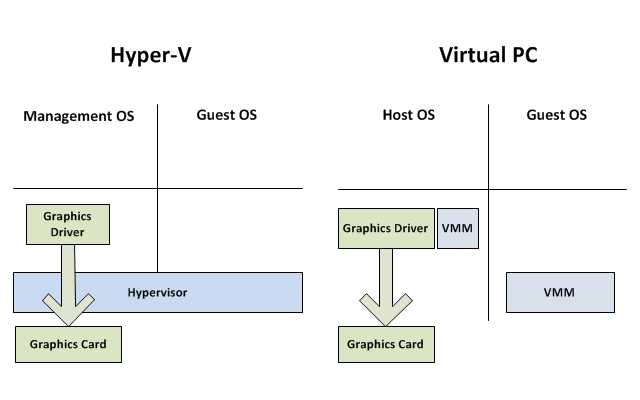
\includegraphics[width=\linewidth]{Comparison.png}
    \end{center}
  \end{figure}
\end{frame}

\begin{frame}{What is a Virtual Environment (\texttt{VE}) / Virtual Machine (\texttt{VM})?}
  \begin{itemize}
    \item Type 2 Environments.
      \begin{itemize}
        \item Virtual Box (Open Source).
        \item Microsoft Virtual \texttt{PC}.
        \item Parallels.
        \item \textbf{VMWare}.
        \item Xen (Open Source).
        \item KVM (Open Source).
      \end{itemize}  
  \end{itemize}
  \begin{block}{NOTE}
    These systems provide \textbf{FULL} Virtualisation.
  \end{block}
\end{frame}

\begin{frame}{Why use \texttt{VM}s?}
  \begin{itemize}
    \item Efficient utilisation of Hardware.
    \item Independence of operation (Sandbox).
      \begin{itemize}
        \item Malware.
        \item Crashes.
        \item Corruption (Failed reboot?).
      \end{itemize}  
    \item For this module
      \begin{itemize}
        \item Portability between lab machines.
        \item Independence from the lab.
      \end{itemize}  
  \end{itemize}  
  \begin{block}{NOTE}
    The simplest environment to provide this is \texttt{VMWare} and there is free version of the player for no-commercial use.
  \end{block}
\end{frame}

\begin{frame}{Issues with \texttt{VM}s?}
  \begin{itemize}
    \item The \texttt{VM}s take up resources on a base operating system.
    \item Virtualised hardware is slower than native hardware.
      \begin{itemize}
        \item Instruction set is emulated so has to be translated and then executed in software which is what actually runs on the hardware.
      \end{itemize}
    \item You have to manage the \texttt{VM} environment as well as the virtualised \texttt{OS}s.
    \item Not all hardware that is emulated may be `shared' by the Host OS and the Virtualised \texttt{OS}.  
  \end{itemize}
\end{frame}

\subsection{How are they used in this module?}
\begin{frame}{Storage of \texttt{VM}s}
  \begin{itemize}
    \item Prepare your drive.
      \begin{itemize}
        \item Two Folders one for the \texttt{VM}s you create and one for the \texttt{ISO} images of the \texttt{OS}s you will install.
        \begin{itemize}
          \item \texttt{VM}
          \item \texttt{ISO}
        \end{itemize}  
      \end{itemize}
    \item Look after your drive you will need it for \textbf{ALL} lab sessions.
  \end{itemize}
\end{frame}

\begin{frame}{Lab Info}
  \begin{itemize}
    \item A basic pre-installed image of \texttt{Ubuntu Server} will be available in the lab and an \texttt{ISO} image of the installer. 
      \begin{itemize}
        \item \texttt{//nas3} or \texttt{//nas3.offcampusnetwork.co.uk} 
      \end{itemize}
    \item Although a basic image is provided you should become comfortable installing the \texttt{OS} from scratch.
  \end{itemize}
  \begin{block}{NOTE}
    This module is based around \texttt{Ubuntu Server} the client you build and use is only to access the infrastructure you build, it is not part of the assessment.
  \end{block}
\end{frame}

\begin{frame}{And finally!}
  \begin{itemize}
    \item Sign out \texttt{USB HDD} a for the storage of your Virtual Machines.
      \begin{itemize}
        \item \texttt{https://orb.northumbria.ac.uk} 
        \item Check the format!
      \end{itemize}
  \end{itemize}
  \begin{block}{NOTE}
    The workshop is to get you to familiarise \textbf{yourself} with \texttt{VMWare}. You may well have to do a bit of research yourself. (Your Second Year \texttt{BSc} students now)
  \end{block}
\end{frame}


% Placing a * after \section means it will not show in the
% outline or table of contents.  

\section*{Summary}

\begin{frame}{Summary}
  \begin{itemize}
    \item What is the module about?
    \item How is it assessed?
    \item What are the resources?
    \item Why do we use virtualisation?
  \end{itemize}
\end{frame}

\end{document}


